% !TeX program = xelatex
\documentclass[UTF8,a4paper,11pt]{ctexart}
\usepackage[left=18mm,right=18mm,top=18mm,bottom=18mm]{geometry}
\usepackage{graphicx}
\usepackage{booktabs}
\usepackage{tabularx}
\usepackage{array}
\usepackage{enumitem}
\usepackage[table]{xcolor}
\usepackage{fancyhdr}
\usepackage{hyperref}
\usepackage{lastpage}

\definecolor{rapidblue}{HTML}{1F5A7A}
\definecolor{rapidcyan}{HTML}{2D91B5}
\definecolor{lightblue}{HTML}{EAF4F8}
\definecolor{warn}{HTML}{FFF1D6}
\definecolor{ink}{HTML}{263238}
\hypersetup{colorlinks=true,linkcolor=rapidblue,urlcolor=rapidcyan,pdfauthor={RapidHand Project},pdftitle={Camera Finger and Thumb BOM and Assembly Guide}}
\setlength{\parindent}{0pt}
\setlength{\parskip}{4pt}
\renewcommand{\arraystretch}{1.32}
\pagestyle{fancy}
\fancyhf{}
\fancyhead[L]{\color{rapidblue}\small RAPID-Hand 相机指端组件}
\fancyhead[R]{\color{rapidblue}\small BOM 与装配指南}
\fancyfoot[L]{\scriptsize 来源：SolidWorks 顶层装配“默认”配置}
\fancyfoot[R]{\scriptsize 第 \thepage\ 页 / 共 \pageref{LastPage} 页}
\renewcommand{\headrulewidth}{0.5pt}

\newcommand{\sectionbar}[1]{%
  \vspace{2pt}\colorbox{rapidblue}{\parbox{\dimexpr\linewidth-2\fboxsep}{\color{white}\Large\bfseries #1}}\vspace{6pt}}
\newcommand{\note}[1]{\colorbox{lightblue}{\parbox{\dimexpr\linewidth-2\fboxsep}{#1}}}
\newcommand{\warningbox}[1]{\colorbox{warn}{\parbox{\dimexpr\linewidth-2\fboxsep}{\textbf{注意：}#1}}}
\newcommand{\checkbox}{\raisebox{.15ex}{\fbox{\rule{0pt}{1.05ex}\rule{1.05ex}{0pt}}}}
\newcolumntype{Y}{>{\raggedright\arraybackslash}X}
\newcolumntype{C}[1]{>{\centering\arraybackslash}p{#1}}

\begin{document}

\begin{titlepage}
  \pagecolor{lightblue}
  \color{ink}
  \vspace*{18mm}
  {\Huge\bfseries RAPID-Hand\par}
  \vspace{4mm}
  {\color{rapidblue}\rule{\linewidth}{2.2pt}}
  \vspace{10mm}
  {\fontsize{26}{32}\selectfont\bfseries 相机手指与相机拇指\par}
  \vspace{3mm}
  {\fontsize{22}{28}\selectfont BOM 与装配指南\par}
  \vspace{12mm}
  \begin{center}
    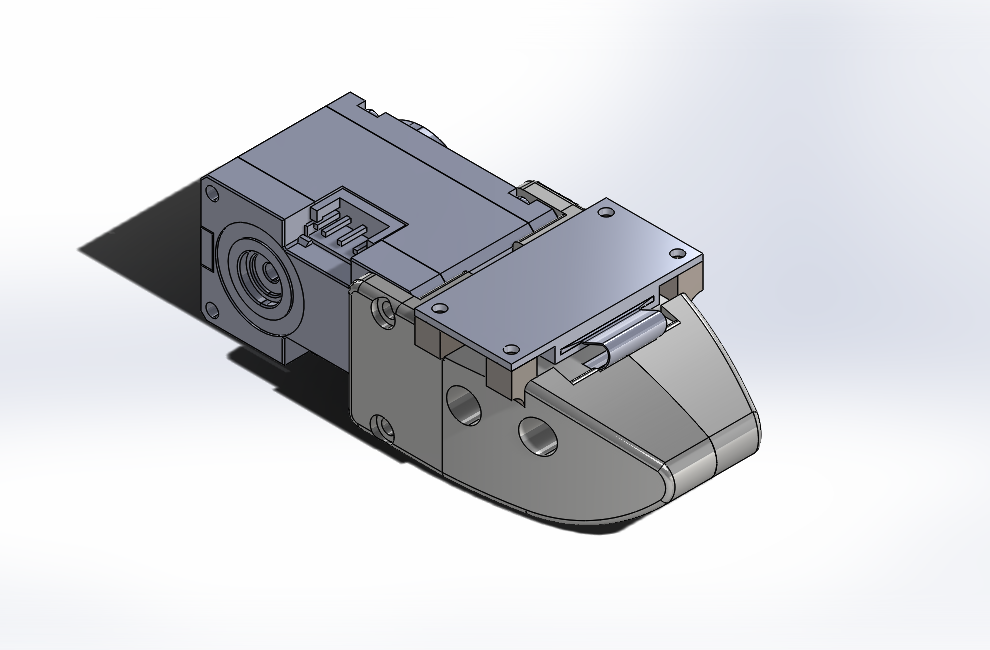
\includegraphics[width=.82\linewidth,trim=45 40 45 35,clip]{figures/thumb_with_cam_isometric.png}
  \end{center}
  \vfill
  \begin{tabularx}{\linewidth}{@{}>{\bfseries}p{40mm}Y@{}}
    适用模型 & \texttt{rss\_design/finger\_with\_cam}；\texttt{rss\_design/thumb\_with\_cam}\\
    数据来源 & SolidWorks 2024 顶层装配树与当前模型视图\\
    文档版本 & 1.0（2026-09-16）\\
  \end{tabularx}
  \vspace{8mm}
\end{titlepage}
\nopagecolor

\sectionbar{1\quad 使用范围与读图约定}

本指南参照原 \texttt{BOM\_and\_Assembly\_Guide.pdf} 的“分类 BOM + 爆炸/装配视图”结构，针对两套带相机的指端子装配单独整理。BOM 数量来自 SolidWorks 顶层装配树，不包含更高层级手掌、关节或线束。

\begin{tabularx}{\linewidth}{@{}p{34mm}Y@{}}
\toprule
\rowcolor{rapidblue}\color{white}\bfseries 项目 & \color{white}\bfseries 约定\\
\midrule
配置 & 两套装配均读取“默认”配置；所有列出的组件均未被抑制。\\
数量 & 统计顶层实例数量；同名紧固件按实例合并。\\
颜色 & 颜色仅用于识别。手指图中蓝色为 M2×4，红色为 M2.5×12。\\
尺寸 & 截图不可用于量取尺寸；加工与打印以原始 SolidWorks 文件为准。\\
紧固件 & 拇指装配未建模紧固件，因此本指南不推断螺钉规格与数量。\\
\bottomrule
\end{tabularx}

\vspace{3mm}
\note{\textbf{建议工具：}公制内六角工具、塑料镊子、低强度可拆卸螺纹锁固剂（按项目规范选用）、无尘布。相机与执行器接插件应按防静电要求操作。}

\warningbox{装配前检查打印件无翘曲、孔内无残余支撑；相机排线不得夹在壳体结合面内。任何阻力异常时先拆检，不要强行锁紧。}

\vfill
\begin{center}
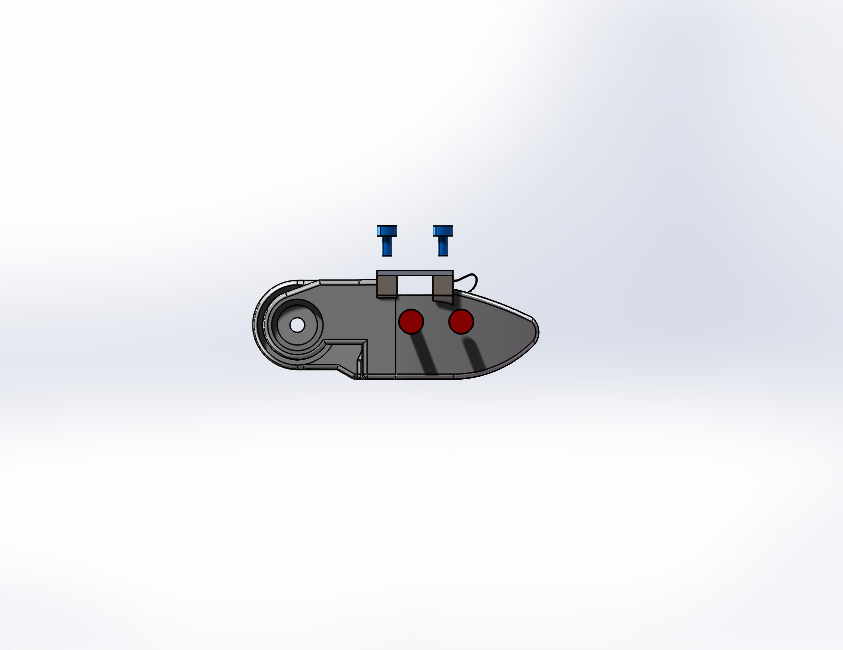
\includegraphics[width=.49\linewidth,trim=40 55 40 40,clip]{figures/finger_with_cam_front.png}\hfill
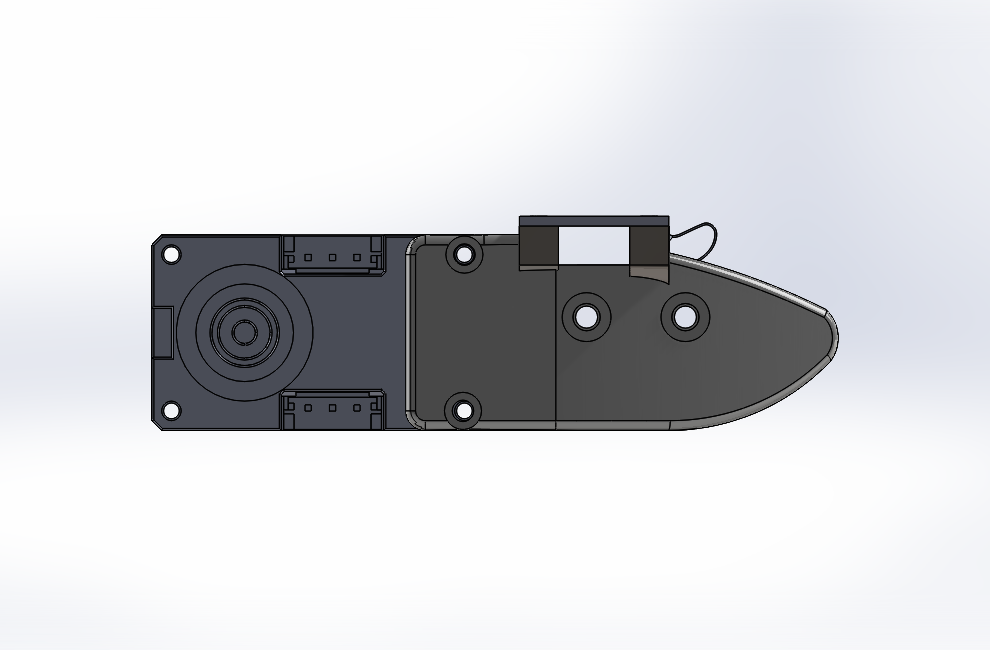
\includegraphics[width=.49\linewidth,trim=40 55 40 40,clip]{figures/thumb_with_cam_front.png}

{\small 图 1\quad SolidWorks 正视图：相机手指（左）与相机拇指（右）}
\end{center}

\clearpage
\sectionbar{2\quad 相机手指 BOM}

\begin{tabularx}{\linewidth}{@{}C{12mm}Y C{15mm} C{23mm} Y@{}}
\toprule
\rowcolor{rapidblue}\color{white}\bfseries 编号 & \color{white}\bfseries 模型文件 & \color{white}\bfseries 数量 & \color{white}\bfseries 分类 & \color{white}\bfseries 说明\\
\midrule
F-01 & \texttt{f1-CamtipR.SLDPRT} & 1 & 结构件 & 右侧相机指尖壳体\\
F-02 & \texttt{f2-CamTipL.SLDPRT} & 1 & 结构件 & 左侧相机指尖壳体\\
F-03 & \texttt{camera.SLDPRT} & 1 & 电子器件 & 指尖相机模型\\
F-04 & \texttt{m2\_4.SLDPRT} & 4 & 标准件 & M2×4 螺钉\\
F-05 & \texttt{m2.5\_12.SLDPRT} & 2 & 标准件 & M2.5×12 螺钉\\
\midrule
 & \textbf{顶层实例合计} & \textbf{9} & & 与装配树一致\\
\bottomrule
\end{tabularx}

\vspace{6mm}
\begin{center}
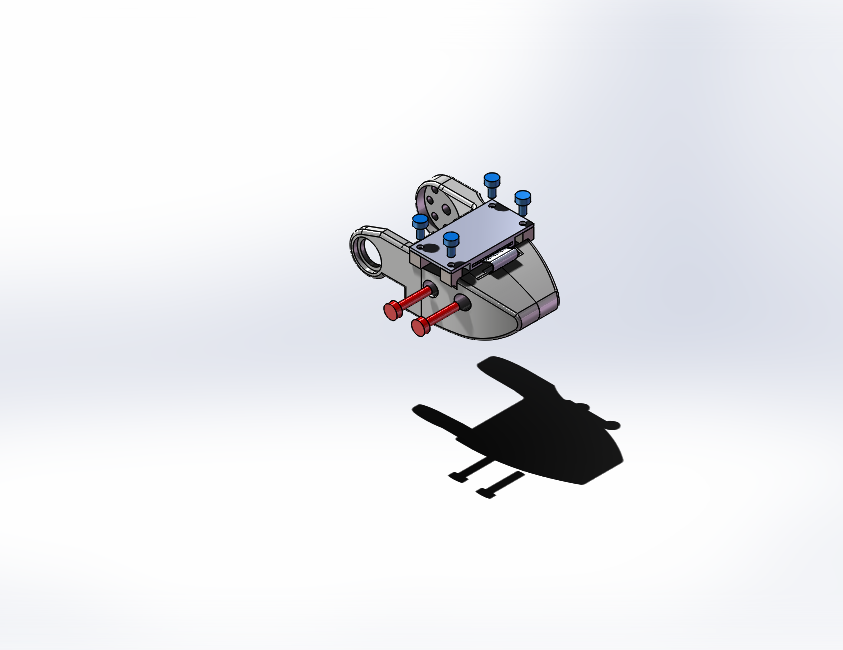
\includegraphics[width=.91\linewidth,trim=85 70 85 55,clip]{figures/finger_with_cam_isometric.png}

{\small 图 2\quad 相机手指等轴测分解状态（SolidWorks 2024 导出）}
\end{center}

\note{\textbf{识别提示：}两枚红色长螺钉为 F-05；四枚蓝色短螺钉为 F-04。相机及上部安装板位于两片壳体之间，线缆从上方槽口引出。}

\clearpage
\sectionbar{3\quad 相机手指装配步骤}

\begin{enumerate}[leftmargin=8mm,label=\textbf{\arabic*.},itemsep=5pt]
  \item \textbf{清理与试配。}检查 F-01、F-02 的结合面、沉孔和相机腔体；先不装螺钉进行干涉试配。
  \item \textbf{安装相机。}将 F-03 镜头朝向指尖外侧的圆形开口，确认镜头中心与开口同轴；排线沿上部槽口自然引出，不得急折。
  \item \textbf{合拢壳体。}以一侧壳体为基准放置相机，再合上另一侧壳体。确认周边接缝贴合，相机不会在腔内晃动。
  \item \textbf{装入 F-05。}将 2 枚 M2.5×12 螺钉装入侧向贯穿位置，仅旋入至刚好接触，不立即锁紧。
  \item \textbf{装入 F-04。}将 4 枚 M2×4 螺钉装入上部四角位置，按对角顺序逐步锁紧。
  \item \textbf{最终紧固与复检。}交替锁紧 F-05；确认壳体不变形、相机视场无遮挡、线缆可自由进入后续走线路径。
\end{enumerate}

\begin{center}
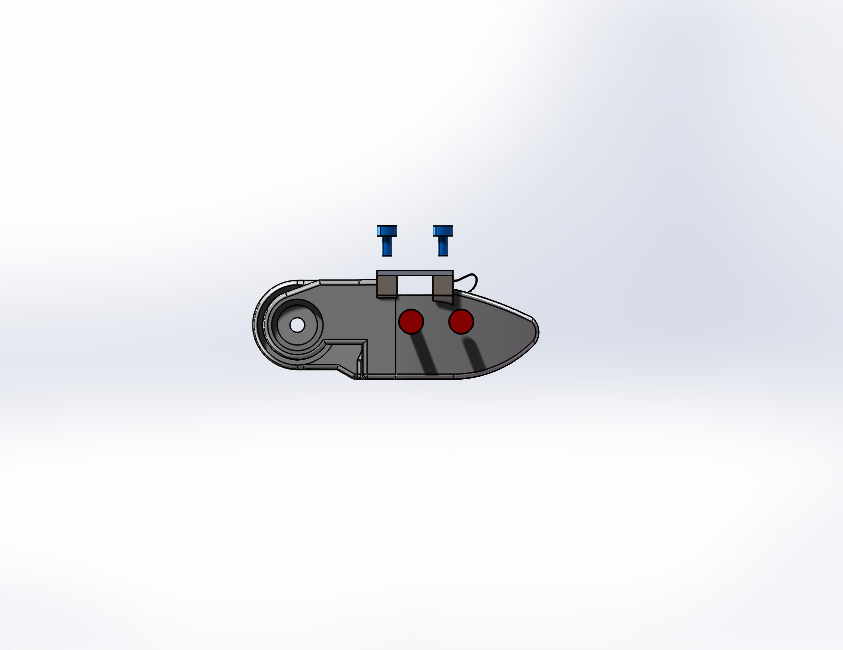
\includegraphics[width=.49\linewidth,trim=55 80 55 55,clip]{figures/finger_with_cam_front.png}\hfill
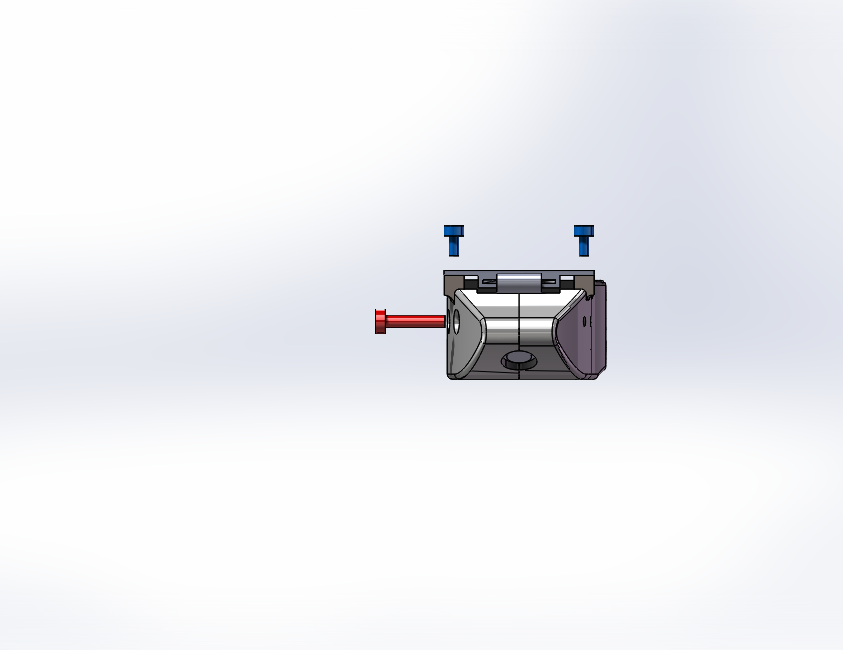
\includegraphics[width=.49\linewidth,trim=55 80 55 55,clip]{figures/finger_with_cam_right.png}

{\small 图 3\quad 锁紧位置核对：正视图（左）与右视图（右）}
\end{center}

\warningbox{M2×4 与 M2.5×12 不可互换。若螺钉在壳体未贴合前已到底，应立即停止并核对孔位、螺纹与零件方向。}

\clearpage
\sectionbar{4\quad 相机拇指 BOM}

\begin{tabularx}{\linewidth}{@{}C{12mm}Y C{15mm} C{23mm} Y@{}}
\toprule
\rowcolor{rapidblue}\color{white}\bfseries 编号 & \color{white}\bfseries 模型文件 & \color{white}\bfseries 数量 & \color{white}\bfseries 分类 & \color{white}\bfseries 说明\\
\midrule
T-01 & \texttt{拇指带摄像头右改.SLDPRT} & 1 & 结构件 & 右侧拇指相机壳体\\
T-02 & \texttt{拇指带摄像头左.SLDPRT} & 1 & 结构件 & 左侧拇指相机壳体\\
T-03 & \texttt{camera.SLDPRT} & 1 & 电子器件 & 拇指指端相机模型\\
T-04 & \texttt{XL,XC-330.SLDPRT} & 1 & 电子器件 & XL/XC-330 执行器模型\\
\midrule
 & \textbf{顶层实例合计} & \textbf{4} & & 与装配树一致\\
\bottomrule
\end{tabularx}

\vspace{6mm}
\begin{center}
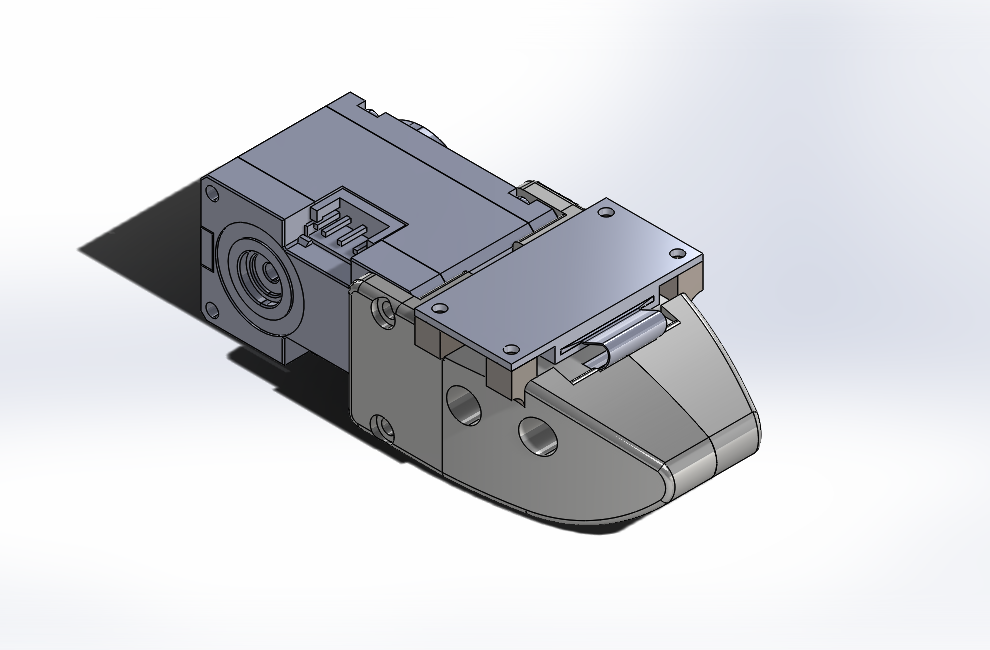
\includegraphics[width=.94\linewidth,trim=45 35 45 30,clip]{figures/thumb_with_cam_isometric.png}

{\small 图 4\quad 相机拇指等轴测装配视图（SolidWorks 2024 导出）}
\end{center}

\warningbox{该 \texttt{SLDASM} 顶层装配不含任何紧固件实例。采购和装配前，必须依据上级总装、工程图或项目紧固件规范补充螺钉/螺母，不应从截图估算规格。}

\clearpage
\sectionbar{5\quad 相机拇指装配步骤}

\begin{enumerate}[leftmargin=8mm,label=\textbf{\arabic*.},itemsep=5pt]
  \item \textbf{确认方向。}指尖圆形镜头孔为远端；执行器方形壳体与圆形输出轴区域为近端。
  \item \textbf{放置执行器。}以 T-01 为基准，将 T-04 放入近端矩形安装腔，使输出轴与壳体圆形轴孔同轴，接插件朝向预留走线空间。
  \item \textbf{安装相机。}将 T-03 放入远端腔体，镜头正对指尖圆孔；让线缆沿上方出口形成自然弯曲，避免压在尖角上。
  \item \textbf{合拢壳体。}装上 T-02，先手压检查整个结合面是否贴合；若出现间隙，重点检查相机排线和执行器接插件位置。
  \item \textbf{按项目规范固定。}使用经工程图或上级 BOM 确认的紧固件完成固定。紧固件尚未确认时，不执行带扭矩的最终锁紧。
  \item \textbf{功能检查。}手动确认输出轴区域无干涉；通电前检查相机镜头无遮挡、线缆无夹伤、连接器极性正确。
\end{enumerate}

\begin{center}
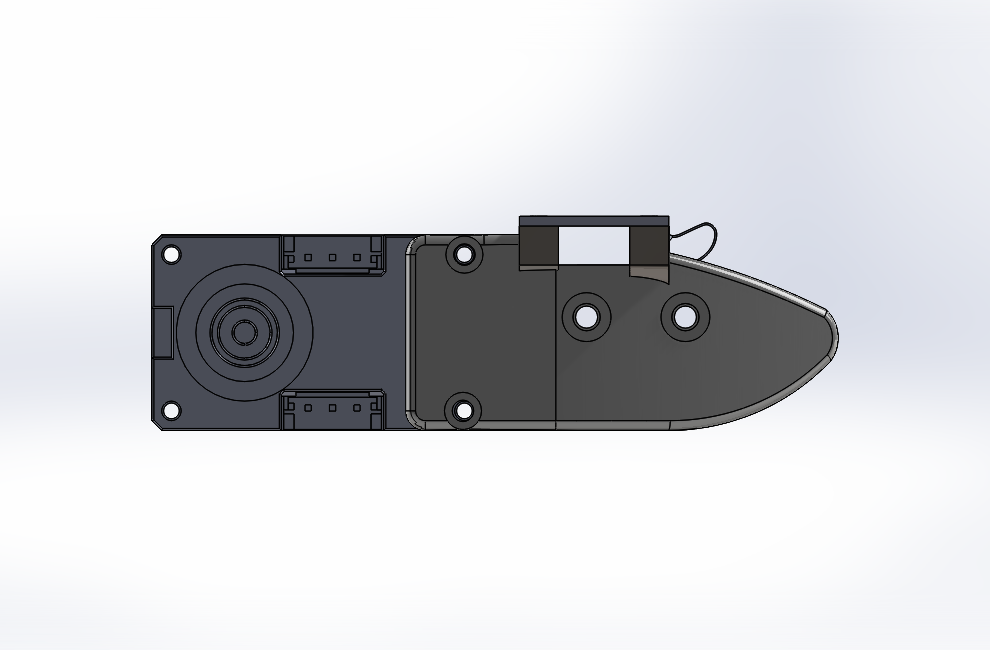
\includegraphics[width=.49\linewidth,trim=45 65 45 45,clip]{figures/thumb_with_cam_front.png}\hfill
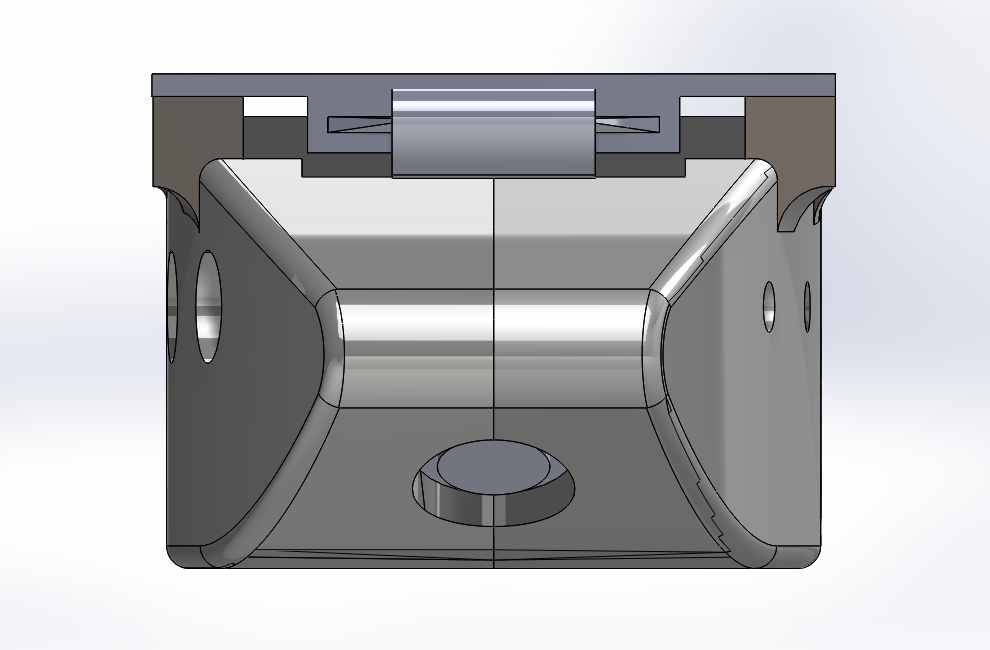
\includegraphics[width=.49\linewidth,trim=45 65 45 45,clip]{figures/thumb_with_cam_right.png}

{\small 图 5\quad 位置核对：正视图（左）与右视图（右）}
\end{center}

\note{\textbf{关键对齐：}执行器输出轴与壳体轴孔同轴；相机镜头与远端圆孔同轴；两条线缆均从设计槽口离开壳体，结合面内不得出现被压线段。}

\clearpage
\sectionbar{6\quad 装配后检验与追溯}

\begin{tabularx}{\linewidth}{@{}C{11mm}Y C{25mm}@{}}
\toprule
\rowcolor{rapidblue}\color{white}\bfseries 序号 & \color{white}\bfseries 检验项目 & \color{white}\bfseries 记录\\
\midrule
1 & BOM 数量与实物逐项核对；手指 9 个顶层实例，拇指 4 个顶层实例。 & \checkbox\ 合格\\
2 & 壳体结合面连续贴合，无明显错位、翘曲或裂纹。 & \checkbox\ 合格\\
3 & 相机镜头居中且无遮挡，保护面无指纹与划伤。 & \checkbox\ 合格\\
4 & 相机与执行器线缆无夹伤、急折或拉紧，连接器方向正确。 & \checkbox\ 合格\\
5 & 手指螺钉规格及数量正确，紧固后壳体未变形。 & \checkbox\ 合格\\
6 & 拇指所用紧固件已有工程依据并补录至制造 BOM。 & \checkbox\ 合格\\
7 & 相机图像、执行器零位与活动范围通过上电测试。 & \checkbox\ 合格\\
\bottomrule
\end{tabularx}

\vspace{8mm}
\begin{tabularx}{\linewidth}{@{}>{\bfseries}p{42mm}Y@{}}
\toprule
模型根目录 & \path{RAPID-Hand-main/RapidHandHardware/mechanical_structure/rss_design}\\
手指主装配 & \texttt{finger\_with\_cam/手指带摄像头.SLDASM}\\
拇指主装配 & \texttt{thumb\_with\_cam/拇指带摄像头.SLDASM}\\
截图生成方式 & SolidWorks 2024 API；标准等轴测、正视与右视；Zoom to Fit 后导出 PNG\\
BOM 生成方式 & 读取顶层 \texttt{AssemblyDoc.GetComponents(false)}，按模型文件名汇总\\
\bottomrule
\end{tabularx}

\vfill
\warningbox{本指南反映上述模型在文档生成时的状态。CAD 更新后应重新导出 BOM 与截图，并复核本指南；本文件不能替代经批准的工程图、公差和扭矩规范。}

\end{document}
